\documentclass[11pt,oneside]{article}
\usepackage[a4paper,margin=25mm,headheight=15pt]{geometry}
\usepackage[T1]{fontenc}
\usepackage[utf8]{inputenc}
\IfFileExists{libertinus.sty}{\usepackage{libertinus}}{\usepackage{lmodern}}
\usepackage{microtype}
\usepackage{amsmath,amssymb,amsthm,mathtools,mathrsfs,bm}
\usepackage{booktabs,longtable,tabularx,array,multirow}
\usepackage{graphicx}
\usepackage{xcolor}
\usepackage{enumitem}
\usepackage{fancyhdr}
\usepackage{titlesec}
\usepackage{listings}
\usepackage{xurl}
\usepackage{hyperref}
\usepackage[nameinlink,noabbrev]{cleveref}

\definecolor{linkblue}{RGB}{24,73,126}
\definecolor{proofgreen}{RGB}{21,100,66}
\definecolor{conditionalorange}{RGB}{161,83,11}
\definecolor{conjecturered}{RGB}{150,34,34}
\definecolor{shadegray}{RGB}{246,247,249}
\definecolor{rulegray}{RGB}{190,196,204}
\hypersetup{
  colorlinks=true,
  linkcolor=linkblue,
  citecolor=proofgreen,
  urlcolor=linkblue,
  pdftitle={Integral, Transform, and Fractional-Calculus Frontiers for the Fabius--Rvachev System},
  pdfsubject={Antiderivatives, definite integrals, inverse Fabius quantiles, fractional calculus, Cauchy transforms, and Jacobi fractions},
  pdfkeywords={Fabius function, Rvachev up-function, inverse Fabius function, fractional calculus, Mellin transform, Cauchy transform, Jacobi continued fraction, order statistics}
}

\pagestyle{fancy}
\fancyhf{}
\fancyhead[L]{\small Integral and fractional-calculus frontiers}
\fancyhead[R]{\small\nouppercase{\leftmark}}
\fancyfoot[C]{\thepage}
\renewcommand{\headrulewidth}{0.4pt}
\titleformat{\section}{\Large\bfseries}{\thesection}{0.7em}{}
\titleformat{\subsection}{\large\bfseries}{\thesubsection}{0.7em}{}
\titleformat{\subsubsection}{\normalsize\bfseries}{\thesubsubsection}{0.7em}{}
\setcounter{secnumdepth}{3}
\setcounter{tocdepth}{2}
\setlist[itemize]{leftmargin=2em,itemsep=0.25em,topsep=0.4em}
\setlist[enumerate]{leftmargin=2.35em,itemsep=0.25em,topsep=0.4em}
\setlength{\emergencystretch}{3em}
\allowdisplaybreaks[2]
\numberwithin{equation}{section}

\newtheorem{theorem}{Theorem}[section]
\newtheorem{proposition}[theorem]{Proposition}
\newtheorem{lemma}[theorem]{Lemma}
\newtheorem{corollary}[theorem]{Corollary}
\newtheorem{identity}[theorem]{Identity}
\newtheorem{conjecture}[theorem]{Conjecture}
\theoremstyle{definition}
\newtheorem{definition}[theorem]{Definition}
\newtheorem{example}[theorem]{Example}
\newtheorem{problem}[theorem]{Frontier problem}
\newtheorem{obligation}[theorem]{Formalization obligation}
\theoremstyle{remark}
\newtheorem{remark}[theorem]{Remark}
\newtheorem{warning}[theorem]{Warning}

\newcommand{\R}{\mathbb R}
\newcommand{\C}{\mathbb C}
\newcommand{\N}{\mathbb N}
\newcommand{\Z}{\mathbb Z}
\newcommand{\E}{\mathbb E}
\newcommand{\Prob}{\mathbb P}
\newcommand{\Var}{\operatorname{Var}}
\newcommand{\Up}{\operatorname{up}}
\newcommand{\sinc}{\operatorname{sinc}}
\newcommand{\supp}{\operatorname{supp}}
\newcommand{\pv}{\operatorname{p.v.}}
\newcommand{\e}{\mathrm e}
\newcommand{\ii}{\mathrm i}
\newcommand{\dd}{\,\mathrm d}
\newcommand{\bigO}{\mathcal O}
\newcommand{\smallo}{o}
\newcommand{\eps}{\varepsilon}
\newcommand{\fall}[2]{#1^{\underline{#2}}}
\newcommand{\rising}[2]{(#1)_{#2}}
\newcommand{\BetaInc}{\mathrm B}
\newcommand{\Gammaf}{\Gamma}
\newcommand{\Mellin}{\mathcal M}
\newcommand{\Laplace}{\mathcal L}
\newcommand{\Fourier}{\mathcal F}
\newcommand{\RLInt}[1]{I_{0+}^{#1}}
\newcommand{\RLIntm}[1]{I_{-1+}^{#1}}
\newcommand{\RLDer}[1]{D_{0+}^{#1}}
\newcommand{\CapDer}[1]{{}^{\mathrm C}\!D_{0+}^{#1}}
\newcommand{\RieszDer}[1]{D_{\mathrm R}^{#1}}
\newcommand{\QF}{Q}
\newcommand{\repo}{\nolinkurl{Analysis/FabiusFunction/docs}}
\newcommand{\statusbackground}{\textcolor{linkblue}{\textbf{Background / corpus result.}}}
\newcommand{\statusproved}{\textcolor{proofgreen}{\textbf{Proved in this report.}}}
\newcommand{\statusconditional}{\textcolor{conditionalorange}{\textbf{Conditional statement.}}}
\newcommand{\statusconjecture}{\textcolor{conjecturered}{\textbf{Conjectural.}}}

\newenvironment{statusbox}{%
  \par\smallskip\noindent\begin{center}\begin{minipage}{0.94\textwidth}%
  \hrule\vspace{0.65em}\small
}{%
  \vspace{0.65em}\hrule\end{minipage}\end{center}\smallskip
}

\lstdefinestyle{reportcode}{
  basicstyle=\ttfamily\footnotesize,
  backgroundcolor=\color{shadegray},
  frame=single,
  rulecolor=\color{rulegray},
  columns=fullflexible,
  keepspaces=true,
  showstringspaces=false,
  breaklines=true,
  xleftmargin=0.7em,
  xrightmargin=0.7em,
  aboveskip=0.8em,
  belowskip=0.8em
}

\title{\bfseries Integral, Transform, and Fractional-Calculus Frontiers\\
for the Fabius--Rvachev System\\[0.45em]
\large Exact kernel formulae, inverse-quantile calculus, Cauchy renormalization,\\
and a Jacobi continued fraction for Rvachev's up-law}
\author{Research report prepared for Vladimir Reshetnikov's \texttt{ProveIt} project}
\date{27 August 2026\\
\small Recursive corpus audit anchored at commit \texttt{32d6d36c51d803289e6d6a0dc0c37753766eba47},\\
with current living manuscripts and active frontier drafts rechecked on the same date}

\begin{document}
\maketitle

\begin{abstract}
The Fabius--Rvachev documentation corpus already contains a mature theory of the
Thue--Morse sequence, the bounded Fabius function, Rvachev's compactly supported
up-function, exact dyadic values, repeated integration, infinite sinc products,
$q$-binomial acceleration, and lower-Lambert endpoint asymptotics.  This report
performs a non-duplication audit of that recursive LaTeX corpus and develops an
integral calculus that joins several structures not previously assembled there.

The main exact device is probabilistic.  If
\(X=\sum_{k\ge1}2^{-k}U_k\), where the \(U_k\) are independent uniform
variables on \([0,1]\), then the bounded Fabius function \(F\) is the distribution
function of \(X\), while on \([0,1]\),
\(\Up(x)=1-F(x)=\Prob(X>x)\).  This converts weighted integrals of \(F\)
and \(\Up\) into expectations of primitives and truncated powers.  It yields
closed forms for monomial weights, exponential kernels, Mellin transforms, all
integer repeated antiderivatives, and fractional Riemann--Liouville integrals.
For \(p>-1\) and \(\alpha>0\), the fractional antiderivatives of
\(x^pF(x)\) and \(x^p\Up(x)\) are expressed by incomplete beta kernels; at
the endpoint they become convergent series in generalized moments
\(m(s)=\E X^s\).  Reflection of the Fabius law gives an entire Newton series
\(m(s)=\sum_{n\ge0}(-1)^n\binom{s}{n}m_n\), thereby covering fractional and
negative powers by rational integer moments.

For the inverse Fabius function \(Q=F^{-1}\), a layer-cake formula gives its
ordinary and fractional antiderivatives, Laplace/Fourier transforms, mixed
Mellin identities, and all quantile moments.  A particularly direct bridge is
\[
 \int_0^1\Up(x)^\alpha\dd x
 =\Gamma(\alpha+1)\,(I_{0+}^{\alpha}Q)(1).
\]
For the full up-law, the Cauchy transform
\(S(z)=\int_{-1}^1\Up(t)/(z-t)\dd t\) satisfies the new exact
functional-differential equation
\(S'(z)=2[S(2z+1)-S(2z-1)]\).  Combining this with the rational moment
sequence resolves a continued-fraction direction explicitly posed in an active
repository draft: \(S\) has a symmetric Jacobi fraction with positive rational
coefficients, whose first values are computed exactly and whose limit is
\(1/4\).  Finally, nonlinear power integrals are identified with order
statistics and shown to obey
\(\int_0^1\Up(x)^p\dd x\sim Q(1/p)\).

All theorems designated as proved are supplied with arguments.  Numerical work
is used only as an independent check and is reproduced by the commented Python
program included with the report.  Novelty claims are relative to the audited
repository, not assertions of exhaustive worldwide priority.
\end{abstract}

\begin{statusbox}
\textbf{Status discipline.}
\statusbackground{} marks facts already present in the repository or standard
literature.  \statusproved{} marks deductions proved here and not located in the
audited corpus in the displayed form.  \statusconditional{} requires an explicit
regularity hypothesis.  \statusconjecture{} is an open proposal.  Numerical
agreement never substitutes for proof.
\end{statusbox}

\tableofcontents
\clearpage

% --------------------------------------------------------------------------
\section{Corpus audit and the non-duplication boundary}
\label{sec:audit}

\subsection{Coverage protocol}

The directory \repo{} is a layered research environment rather than a single
paper.  At the pinned 27 August 2026 snapshot, an existing audit inventory
records all 67 distinct \texttt{*.tex} paths.  The archive README explains that
historical files are frozen provenance objects and that byte-identical current
duplicates are pruned.  The non-formalized frontier directory is explicitly a
quarantine boundary: its claims are not silently promoted into the formalized
primary exposition \cite{proveitArchive,proveitFrontierReadme,proveitNewton}.

The present audit used four passes.
\begin{enumerate}
\item The 67-path inventory supplied the recursive coverage scaffold.
\item Living primary manuscripts, the consolidated frontier volume, the
      Thue--Morse atlas, inverse-function reports, repeated-integration reports,
      and every active top-level frontier report were reopened on the current
      branch.
\item Frozen archive entries were compared by mathematical lineage, so that a
      superseded copy did not count as an independent novelty witness, while a
      distinctive historical argument remained part of the boundary.
\item Candidate phrases and neighboring concepts were searched thematically:
      Riemann--Liouville and Caputo calculus, fractional primitives, inverse
      layer-cake formulae, Cauchy and Hilbert transforms, Stieltjes/Jacobi
      fractions, order statistics, power integrals, and generalized negative
      moments.
\end{enumerate}

This procedure located substantial adjacent work.  In particular, the corpus
already contains rational up-moments, Hankel determinants, monic orthogonal
polynomials, Gaussian and Lobatto quadrature, and repeated-integration
hierarchies.  One active report explicitly proposes a Jacobi continued fraction
for the moment generating function or Cauchy transform as a future direction
\cite{proveitQuadrature}.  Therefore the continued fraction below is presented
as a resolution of a recorded gap, not as a topic absent from the research
program.

\subsection{What is imported and what is added}

\begin{center}
\small
\begin{tabularx}{0.98\textwidth}{@{}p{0.22\textwidth}X X@{}}
\toprule
Theme & Existing corpus foundation & Addition in this report \\
\midrule
Probability dictionary
& \(F\) as a smooth distribution function; \(\Up\) as the density of a
symmetric random series; exact Laplace/Fourier products
& Universal survival-kernel calculus for arbitrary weights, including partial
antiderivatives and truncated moments \\
Repeated integration
& Integer repeated-integral formulae and exact derivative towers
& One incomplete-beta theorem interpolating all integer and fractional orders
for \(x^pF\) and \(x^p\Up\) \\
Moments and Bernoulli data
& Rational integer moments from Bernoulli cumulants and Bell recurrences
& Entire Newton interpolation \(m(s)\), Mellin continuation, negative powers,
and logarithmic integrals \\
Inverse Fabius
& Dyadic inverse germs, Richardson acceleration, endpoint Lambert--Gamma--zeta
asymptotics, inverse elasticity
& Layer-cake transforms, quantile antiderivatives, mixed Mellin identities, and
fractional \(Q\)-calculus \\
Orthogonal polynomials
& Hankel norms and positive Gaussian quadrature; J-fraction posed as an open
problem
& Cauchy renormalization equation, explicit symmetric J-fraction, exact rational
coefficients, and the \(1/4\) limit \\
Nonlinear integrals
& Endpoint/inverse asymptotics sufficient to prove slow variation of \(Q\)
& Order-statistic formulae and \(\int\Up^p\sim Q(1/p)\), with a second-order
frontier conjecture \\
Fractional derivatives
& No Riemann--Liouville/Caputo treatment located
& Exact fractional refinement equations for \(F\), \(\Up\), and \(Q\), plus a
full-line Riesz refinement law \\
\bottomrule
\end{tabularx}
\end{center}

\begin{remark}[Priority boundary]
The formulae below often use classical probability, Mellin, fractional-calculus,
and orthogonal-polynomial tools.  The novelty assertion is the corpus-relative
combination and the displayed Fabius--Rvachev specializations.  A worldwide
priority claim would require a dedicated multilingual search using all historical
normalizations of the Fabius and up-functions.
\end{remark}

% --------------------------------------------------------------------------
\section{Normalizations and the probabilistic platform}
\label{sec:platform}

\subsection{The bounded Fabius law and the up-law}

Let \(U_1,U_2,\ldots\) be independent and uniformly distributed on \([0,1]\), and
put
\begin{equation}
 X=\sum_{k=1}^{\infty}\frac{U_k}{2^k}.
 \label{eq:Xdef}
\end{equation}
Then \(0<X<1\) almost surely.  Let
\begin{equation}
 F(x)=\Prob(X\le x),\qquad 0\le x\le1,
 \label{eq:Fcdf}
\end{equation}
and extend it by \(F(x)=0\) for \(x<0\), \(F(x)=1\) for \(x>1\).
This is the bounded Fabius function in the normalization used throughout the
repository.  It is a strictly increasing \(C^\infty\) bijection of \([0,1]\),
flat at both endpoints, and satisfies
\begin{equation}
 F(1-x)=1-F(x),
 \qquad
 F'(x)=2\Up(2x-1).
 \label{eq:Fuprelations}
\end{equation}

Let \(V_k=2U_k-1\), uniform on \([-1,1]\), and define
\begin{equation}
 Y=2X-1=\sum_{k=1}^{\infty}\frac{V_k}{2^k}.
 \label{eq:Ydef}
\end{equation}
The density of \(Y\) is Rvachev's even up-function \(\Up\), supported on
\([-1,1]\), normalized by \(\int\Up=1\) and \(\Up(0)=1\).  On the positive half
of its support,
\begin{equation}
 \boxed{\Up(x)=F(1-x)=1-F(x)=\Prob(X>x),\qquad 0\le x\le1.}
 \label{eq:up-survival}
\end{equation}
Thus the right half of the up-bump is exactly the survival function of the
Fabius probability law.

The fixed-point decompositions
\begin{equation}
 X\stackrel d=\frac{U+X'}2,
 \qquad
 Y\stackrel d=\frac{V+Y'}2
 \label{eq:fixedpoints}
\end{equation}
use independent copies \(X',Y'\).  They imply
\begin{equation}
 \Up'(x)=2\bigl(\Up(2x+1)-\Up(2x-1)\bigr)
 \label{eq:up-refinement}
\end{equation}
and, on \(0<x<1/2\), \(F'(x)=2F(2x)\).  These are established corpus
identities \cite{proveitPrimary,arias1982}.

\subsection{Entire exponential products and rational cumulants}

Define
\begin{align}
 A(z)&=\E\e^{zX}
 =\prod_{k=1}^{\infty}\frac{\e^{z/2^k}-1}{z/2^k},
 \label{eq:Aproduct}\\
 \Phi(z)&=\E\e^{zY}
 =\e^{-z}A(2z)
 =\prod_{k=1}^{\infty}\frac{\sinh(z/2^k)}{z/2^k}.
 \label{eq:PhiProduct}
\end{align}
Both are entire.  With Bernoulli numbers in the convention \(B_1=-1/2\), the
cumulants of \(X\) are
\begin{equation}
 \kappa_1(X)=\frac12,
 \qquad
 \boxed{\kappa_n(X)=\frac{B_n}{n(2^n-1)},\quad n\ge2,}
 \label{eq:Xcumulants}
\end{equation}
and those of \(Y\) are
\begin{equation}
 \kappa_1(Y)=0,
 \qquad
 \boxed{\kappa_n(Y)=\frac{2^nB_n}{n(2^n-1)},\quad n\ge2.}
 \label{eq:Ycumulants}
\end{equation}
Consequently all integer moments are rational and are generated by complete
Bell polynomials:
\begin{equation}
 m_n:=\E X^n=\mathcal B_n(\kappa_1(X),\ldots,\kappa_n(X)),
 \qquad
 \mu_n:=\E Y^n=\mathcal B_n(\kappa_1(Y),\ldots,\kappa_n(Y)).
 \label{eq:BellMoments}
\end{equation}
The first values are
\begin{align}
 (m_0,m_1,m_2,m_3,m_4,m_5,m_6)
 &=\left(1,\frac12,\frac5{18},\frac16,\frac{143}{1350},
 \frac{19}{270},\frac{1153}{23814}\right),
 \label{eq:XmomentsLow}\\
 (\mu_0,\mu_2,\mu_4,\mu_6,\mu_8)
 &=\left(1,\frac19,\frac{19}{675},\frac{583}{59535},
 \frac{132809}{32531625}\right).
 \label{eq:YmomentsLow}
\end{align}

% --------------------------------------------------------------------------
\section{The universal survival-kernel calculus}
\label{sec:survival}

\subsection{Arbitrary kernels and partial antiderivatives}

\begin{theorem}[Survival-kernel identity]
\label{thm:survival-kernel}
Let \(k\in L^1(0,1)\), and put \(K(x)=\int_0^x k(t)\dd t\).  Then
\begin{equation}
 \boxed{\int_0^1 k(t)\Up(t)\dd t=\E K(X).}
 \label{eq:survival-master}
\end{equation}
More generally, for \(0\le x\le1\),
\begin{equation}
 \boxed{\int_0^x k(t)\Up(t)\dd t
 =\E K(\min\{X,x\}).}
 \label{eq:survival-partial}
\end{equation}
Both identities remain valid for complex-valued kernels whenever the displayed
integrals are absolutely convergent.  \statusproved
\end{theorem}

\begin{proof}
By \eqref{eq:up-survival},
\(\Up(t)=\E\mathbf1_{\{t<X\}}\).  Tonelli--Fubini gives
\[
 \int_0^x k(t)\Up(t)\dd t
 =\E\int_0^x k(t)\mathbf1_{\{t<X\}}\dd t
 =\E\int_0^{\min(X,x)}k(t)\dd t.
\]
Taking \(x=1\) proves \eqref{eq:survival-master}.
\end{proof}

\begin{corollary}[Monomial antiderivatives]
\label{cor:monomial-partial}
For \(\Re p>-1\) and \(0\le x\le1\),
\begin{align}
 \int_0^x t^p\Up(t)\dd t
 &=\frac{\E\min(X,x)^{p+1}}{p+1},
 \label{eq:up-monomial-partial}\\
 \int_0^x t^pF(t)\dd t
 &=\frac{x^{p+1}-\E\min(X,x)^{p+1}}{p+1}.
 \label{eq:F-monomial-partial}
\end{align}
At \(x=1\), writing \(m(s)=\E X^s\),
\begin{align}
 \boxed{\int_0^1t^p\Up(t)\dd t=\frac{m(p+1)}{p+1},}
 \label{eq:up-monomial-full}\\
 \boxed{\int_0^1t^pF(t)\dd t=\frac{1-m(p+1)}{p+1}.}
 \label{eq:F-monomial-full}
\end{align}
\statusproved
\end{corollary}

For nonnegative integers, this gives for example
\begin{center}
\begin{tabular}{c|ccc}
\toprule
& \(p=0\) & \(p=1\) & \(p=2\)\\
\midrule
\(\int_0^1x^p\Up(x)\dd x\)
& \(1/2\) & \(5/36\) & \(1/18\)\\
\(\int_0^1x^pF(x)\dd x\)
& \(1/2\) & \(13/36\) & \(5/18\)\\
\bottomrule
\end{tabular}
\end{center}

\begin{remark}[Negative powers]
The survival integral in \eqref{eq:up-monomial-full} has the sharp local
restriction \(\Re p>-1\), because \(\Up(0)=1\).  In contrast, \(F\) is flat at
zero, so \(\int_0^1x^pF(x)\dd x\) converges for every \(p\in\C\); the right side
of \eqref{eq:F-monomial-full} supplies its entire continuation after removing
the apparent singularity at \(p=-1\).  In particular,
\begin{equation}
 \int_0^1\frac{F(x)}x\dd x=-m'(0)=\E[-\log X].
 \label{eq:F-over-x}
\end{equation}
\end{remark}

\subsection{Exponential kernels and ordinary transforms}

Taking \(k(t)=\e^{zt}\) in \cref{thm:survival-kernel} yields the entire
identities
\begin{align}
 \boxed{\int_0^1\Up(t)\e^{zt}\dd t=\frac{A(z)-1}{z},}
 \label{eq:up-exp-transform}\\
 \boxed{\int_0^1F(t)\e^{zt}\dd t=\frac{\e^z-A(z)}{z},}
 \label{eq:F-exp-transform}
\end{align}
with removable values at \(z=0\).  Differentiation under the integral gives all
monomial-exponential combinations:
\begin{align}
 \int_0^1t^n\Up(t)\e^{zt}\dd t
 &=\frac{\dd^n}{\dd z^n}\left(\frac{A(z)-1}{z}\right),
 \label{eq:up-monomial-exp}\\
 \int_0^1t^nF(t)\e^{zt}\dd t
 &=\frac{\dd^n}{\dd z^n}\left(\frac{\e^z-A(z)}{z}\right).
 \label{eq:F-monomial-exp}
\end{align}
At \(z=-2\pi\ii\xi\), these are the finite-interval Fourier transforms of
\(F\) and the positive half of \(\Up\).

\subsection{Derivative-weighted beta integrals}

\begin{theorem}[Probability-integral-transform family]
\label{thm:beta-family}
Let \(a,b\in\C\) with \(\Re a,\Re b>-1\).  Then
\begin{equation}
 \boxed{\int_0^1 F(x)^a(1-F(x))^bF'(x)\dd x
 =\mathrm B(a+1,b+1).}
 \label{eq:F-beta}
\end{equation}
More generally, for any integrable \(\varphi\),
\begin{equation}
 \int_0^1\varphi(F(x))F'(x)\dd x=\int_0^1\varphi(u)\dd u.
 \label{eq:PIT}
\end{equation}
Equivalently, since \(F'(x)=2\Up(2x-1)\), this is an exact family of integrals
mixing the up-function with powers of the Fabius function.  \statusproved
\end{theorem}

\begin{proof}
Use the substitution \(u=F(x)\), legitimate because \(F\) is a smooth strictly
increasing bijection of \([0,1]\).
\end{proof}

The quantile-weighted extension is
\begin{equation}
 \int_0^1x^rF(x)^a(1-F(x))^bF'(x)\dd x
 =\int_0^1\QF(u)^r u^a(1-u)^b\dd u,
 \label{eq:weighted-beta-quantile}
\end{equation}
where \(\QF=F^{-1}\).  Thus every beta-weighted moment of the inverse is a
forward Fabius integral.

% --------------------------------------------------------------------------
\section{Generalized moments and the Mellin transform}
\label{sec:mellin}

\subsection{An entire Newton series from reflection}

The flat endpoints imply more than the existence of all negative moments.

\begin{lemma}[Super-polynomial decay of integer moments]
\label{lem:moment-decay}
For every \(N>0\),
\begin{equation}
 m_n=\E X^n=\bigO_N(n^{-N})\qquad(n\to\infty).
 \label{eq:moment-superpoly}
\end{equation}
\statusproved
\end{lemma}

\begin{proof}
By reflection, \(\Prob(X>1-t)=F(t)\).  Endpoint flatness gives
\(F(t)=\bigO_M(t^M)\) for every \(M\).  The layer-cake formula
\[
 m_n=n\int_0^1x^{n-1}\Prob(X>x)\dd x
\]
followed by \(x=1-t\), a split at fixed small \(t\), and
\((1-t)^{n-1}\le\e^{-(n-1)t}\) gives \(m_n=\bigO_M(n^{-M})\).
\end{proof}

\begin{theorem}[Entire Newton interpolation of Fabius moments]
\label{thm:moment-newton}
For every \(s\in\C\),
\begin{equation}
 \boxed{m(s):=\E X^s
 =\sum_{n=0}^{\infty}(-1)^n\binom{s}{n}m_n.}
 \label{eq:moment-newton}
\end{equation}
The series converges absolutely and locally uniformly in \(s\), hence defines
an entire function.  Its coefficients \(m_n\) are rational Bell polynomials in
the Bernoulli--Mersenne cumulants \eqref{eq:Xcumulants}.  \statusproved
\end{theorem}

\begin{proof}
The reflection law gives \(1-X\stackrel d=X\).  For every fixed \(0<X<1\),
\[
 X^s=(1-(1-X))^s
 =\sum_{n\ge0}(-1)^n\binom{s}{n}(1-X)^n.
\]
On compact subsets of the \(s\)-plane, the generalized binomial coefficients
grow at most polynomially in \(n\), while \cref{lem:moment-decay} makes \(m_n\)
smaller than every inverse power.  Thus expectation and summation may be
interchanged, and local uniform convergence follows.
\end{proof}

Important specializations are
\begin{align}
 m(-r)&=\sum_{n=0}^{\infty}\binom{n+r-1}{n}m_n,
 &&r\in\N,
 \label{eq:negative-moments-series}\\
 -m'(0)&=\sum_{n=1}^{\infty}\frac{m_n}{n},
 \label{eq:log-moment-series}
\end{align}
so \eqref{eq:F-over-x} has a convergent series of rational terms.  Numerically,
\begin{equation}
 \int_0^1\frac{F(x)}x\dd x
 =0.7582399961\ldots,
 \qquad
 \int_0^1\frac{F(x)}{x^2}\dd x
 =m(-1)-1=1.314885\ldots.
 \label{eq:negative-examples}
\end{equation}
The decimals are checks, not claimed closed constants.

\subsection{A three-function Mellin dictionary}

\begin{theorem}[Mellin transform triad]
\label{thm:mellin-triad}
For \(\Re s>0\),
\begin{align}
 \Mellin[\Up|_{[0,1]}](s)
 &=\int_0^1x^{s-1}\Up(x)\dd x
 =\frac{m(s)}s,
 \label{eq:Mellin-up}\\
 \Mellin[F](s)
 &=\int_0^1x^{s-1}F(x)\dd x
 =\frac{1-m(s)}s,
 \label{eq:Mellin-F}\\
 \Mellin[F'](s)
 &=\int_0^1x^{s-1}F'(x)\dd x
 =m(s-1).
 \label{eq:Mellin-density}
\end{align}
The first extends meromorphically to \(\C\) with one simple pole at \(s=0\),
of residue one.  The second and third extend entire.  \statusproved
\end{theorem}

\begin{proof}
The first identity is \eqref{eq:up-monomial-full} with \(p=s-1\).  The second
follows from \(F=1-\Up\), and the third is the definition of expectation under
the density \(F'\).  Entire continuation uses \cref{thm:moment-newton}; the zero
of \(1-m(s)\) at \(s=0\) removes the apparent pole in \eqref{eq:Mellin-F}.
\end{proof}

The Mellin triad isolates a striking analytic asymmetry.  The positive half of
the up-function equals one at the origin and therefore contributes the single
Mellin pole.  The Fabius function and its density are flat there, and their
Mellin transforms are entire.

% --------------------------------------------------------------------------
\section{Inverse Fabius integral calculus}
\label{sec:inverse}

Let
\begin{equation}
 \QF=F^{-1}:[0,1]\to[0,1].
 \label{eq:Qdef}
\end{equation}
It satisfies \(\QF(1-u)=1-\QF(u)\).

\subsection{Area identity and ordinary antiderivatives}

\begin{theorem}[Inverse-area antiderivative]
\label{thm:inverse-area}
For \(0\le u\le1\),
\begin{equation}
 \boxed{\int_0^u\QF(v)\dd v
 =u\QF(u)-\int_0^{\QF(u)}F(x)\dd x.}
 \label{eq:inverse-area}
\end{equation}
In particular, \(\int_0^1\QF(u)\dd u=1/2\).  \statusproved
\end{theorem}

\begin{proof}
The rectangle \([0,\QF(u)]\times[0,u]\) is partitioned, up to the graph, into
the area below \(F\) and the area to the left of \(\QF\).  Equivalently,
substitute \(v=F(x)\) and integrate by parts.
\end{proof}

\subsection{A general layer-cake transform}

\begin{theorem}[Forward--inverse layer cake]
\label{thm:inverse-layercake}
Let \(\phi\in L^1(0,1)\), and let \(\Psi\) be absolutely continuous with
\(\Psi(0)=0\).  Whenever the right side is absolutely integrable,
\begin{equation}
 \boxed{
 \int_0^1\phi(u)\Psi(\QF(u))\dd u
 =\int_0^1\Psi'(x)\left(\int_{F(x)}^1\phi(u)\dd u\right)\dd x.}
 \label{eq:inverse-layercake}
\end{equation}
\statusproved
\end{theorem}

\begin{proof}
Write
\(\Psi(\QF(u))=\int_0^1\Psi'(x)\mathbf1_{\{x<\QF(u)\}}\dd x\).
Since \(x<\QF(u)\) is equivalent to \(F(x)<u\), Fubini gives the result.
\end{proof}

With \(\Psi(x)=x^p\), \(\Re p>0\), this becomes
\begin{equation}
 \int_0^1\phi(u)\QF(u)^p\dd u
 =p\int_0^1x^{p-1}\left(\int_{F(x)}^1\phi(u)\dd u\right)\dd x.
 \label{eq:inverse-power-layercake}
\end{equation}
Taking \(\phi=1\) proves the exact quantile-moment identity
\begin{equation}
 \boxed{\int_0^1\QF(u)^p\dd u=m(p),}
 \qquad \Re p>0,
 \label{eq:quantile-moments}
\end{equation}
with analytic continuation supplied by \cref{thm:moment-newton} where desired.

\subsection{Laplace, Fourier, and mixed Mellin transforms of the inverse}

For \(s\ne0\), \cref{thm:inverse-layercake} with \(\Psi(x)=x\) gives
\begin{equation}
 \boxed{
 \int_0^1\e^{-su}\QF(u)\dd u
 =\frac1s\int_0^1\bigl(\e^{-sF(x)}-\e^{-s}\bigr)\dd x.}
 \label{eq:Q-Laplace}
\end{equation}
Similarly, for \(t\ne0\),
\begin{equation}
 \boxed{
 \int_0^1\e^{\ii tu}\QF(u)\dd u
 =\frac1{\ii t}\int_0^1\bigl(\e^{\ii t}-\e^{\ii tF(x)}\bigr)\dd x.}
 \label{eq:Q-Fourier}
\end{equation}
These identities replace a transform of a difficult inverse by nonlinear but
forward evaluations of \(F\).

A two-parameter Mellin identity follows by taking \(\phi(u)=u^{s-1}\).

\begin{theorem}[Mixed forward--inverse Mellin identity]
\label{thm:mixed-Mellin-Q}
For \(\Re s>0\), \(\Re p>0\),
\begin{equation}
 \boxed{
 \int_0^1u^{s-1}\QF(u)^p\dd u
 =\frac1s-\frac p s\int_0^1x^{p-1}F(x)^s\dd x.}
 \label{eq:mixed-Mellin-Q}
\end{equation}
\statusproved
\end{theorem}

This makes nonlinear powers \(F^s\) and inverse moments two faces of one
transform.  For integer \(s\), the right side has the order-statistic
interpretation developed in \cref{sec:power-integrals}.

\subsection{All ordinary derivatives of the inverse}

Put \(f=F'\), and, after differentiating with respect to the spatial variable
\(x\), define
\begin{equation}
 R_1(x)=\frac1{f(x)},
 \qquad
 R_{n+1}(x)=\frac{R_n'(x)}{f(x)}.
 \label{eq:inverse-derivative-recurrence}
\end{equation}
Then
\begin{equation}
 \boxed{\QF^{(n)}(u)=R_n(\QF(u)),\qquad 0<u<1.}
 \label{eq:inverse-nth-derivative}
\end{equation}
This is simply the operator formula
\begin{equation}
 \QF^{(n)}(u)
 =\left.\left(\frac1{F'(x)}\frac\dd{\dd x}\right)^{n-1}
 \frac1{F'(x)}\right|_{x=\QF(u)}.
 \label{eq:inverse-operator}
\end{equation}
The first cases are
\begin{align}
 \QF'&=f^{-1},
 &\QF''&=-\frac{f'}{f^3},
 \label{eq:Q12}\\
 \QF'''&=\frac{3(f')^2-ff''}{f^5},
 &\QF''''&=\frac{-15(f')^3+10ff'f''-f^2f'''}{f^7},
 \label{eq:Q34}
\end{align}
all evaluated at \(x=\QF(u)\).  The recurrence is preferable to a single large
Fa\`a di Bruno polynomial when high orders are required.

% --------------------------------------------------------------------------
\section{Integer-order derivative and antiderivative hierarchies}
\label{sec:integer-orders}

\subsection{The Thue--Morse derivative tower}

Let \(s_2(j)\) denote the binary digit sum.  Iterating
\eqref{eq:up-refinement} gives the established exact formula
\begin{equation}
 \boxed{
 \Up^{(n)}(x)=2^{n(n+1)/2}
 \sum_{j=0}^{2^n-1}(-1)^{s_2(j)}
 \Up\bigl(2^nx+2^n-1-2j\bigr).}
 \label{eq:up-nth-derivative}
\end{equation}
On the left edge of the Fabius interval,
\begin{equation}
 \boxed{F^{(n)}(x)=2^{n(n+1)/2}F(2^nx),
 \qquad 0\le x\le2^{-n}.}
 \label{eq:F-left-derivative}
\end{equation}
These are imported corpus results; their role here is to connect the integral
formulae to arbitrary derivative order.

For any nonnegative integer \(m\), integration by parts and endpoint flatness
give
\begin{equation}
 \int_{-1}^1x^m\Up^{(n)}(x)\dd x
 =\begin{cases}
 (-1)^n\dfrac{m!}{(m-n)!}\,\mu_{m-n},&m\ge n,\\[0.8em]
 0,&m<n,
 \end{cases}
 \label{eq:up-derivative-moments}
\end{equation}
and, for \(n\ge1\),
\begin{equation}
 \boxed{
 \int_0^1x^pF^{(n)}(x)\dd x
 =(-1)^{n-1}\fall{p}{n-1}\,m(p-n+1),}
 \label{eq:F-derivative-moments}
\end{equation}
initially where the integration-by-parts calculation is classical and then by
analytic continuation.  Exponential weights similarly yield
\begin{align}
 \int_{-1}^1\e^{zx}\Up^{(n)}(x)\dd x&=(-z)^n\Phi(z),
 \label{eq:up-derivative-exp}\\
 \int_0^1\e^{zx}F^{(n)}(x)\dd x&=(-z)^{n-1}A(z),\qquad n\ge1.
 \label{eq:F-derivative-exp}
\end{align}

\subsection{All repeated antiderivatives as truncated moments}

For integer \(n\ge1\),
\begin{align}
 (I_{0+}^{n}F)(x)
 &=\frac1{n!}\E(x-X)_+^n,
 \label{eq:F-integer-primitive}\\
 (I_{-1+}^{n}\Up)(x)
 &=\frac1{(n-1)!}\E(x-Y)_+^{n-1},
 \label{eq:up-integer-primitive}\\
 (I_{0+}^{n}\QF)(u)
 &=\frac1{n!}\int_0^{\QF(u)}(u-F(x))^n\dd x.
 \label{eq:Q-integer-primitive}
\end{align}
The first and third are special cases of fractional theorems below.  For
\(x>1\), the up antiderivative becomes the finite moment polynomial
\begin{equation}
 (I_{-1+}^{n}\Up)(x)
 =\frac1{(n-1)!}
 \sum_{r=0}^{\lfloor(n-1)/2\rfloor}
 \binom{n-1}{2r}\mu_{2r}x^{n-1-2r}.
 \label{eq:up-exterior-polynomial}
\end{equation}
Thus the rational up-moments are precisely the coefficients of all exterior
ordinary antiderivatives.

% --------------------------------------------------------------------------
\section{Fractional calculus}
\label{sec:fractional}

\subsection{Conventions}

For \(\alpha>0\), the left Riemann--Liouville integral is
\begin{equation}
 (I_{a+}^{\alpha}g)(x)
 =\frac1{\Gamma(\alpha)}\int_a^x(x-t)^{\alpha-1}g(t)\dd t.
 \label{eq:RL-definition}
\end{equation}
For \(n-1<\alpha<n\),
\begin{equation}
 D_{a+}^{\alpha}g=\frac{\dd^n}{\dd x^n}I_{a+}^{n-\alpha}g,
 \qquad
 {}^{\mathrm C}D_{a+}^{\alpha}g=I_{a+}^{n-\alpha}g^{(n)}.
 \label{eq:RL-Caputo}
\end{equation}
These conventions follow the standard monograph of Samko, Kilbas, and Marichev
\cite{samko}.  Because \(F\) and \(\Up\) are flat at their relevant left
endpoints, the usual boundary correction terms between Riemann--Liouville and
Caputo derivatives vanish whenever both sides are classically defined.

\subsection{Fractional primitives and derivatives of the Fabius function}

\begin{theorem}[Fractional truncated-power formula for \(F\)]
\label{thm:F-fractional}
For \(\alpha>0\) and real \(x\), with \(F\) extended as a distribution
function,
\begin{equation}
 \boxed{
 (I_{0+}^{\alpha}F)(x)
 =\frac1{\Gamma(\alpha+1)}\E(x-X)_+^{\alpha}.}
 \label{eq:F-fractional-integral}
\end{equation}
For \(0<\alpha<1\) and \(0<x<1\),
\begin{equation}
 \boxed{
 (D_{0+}^{\alpha}F)(x)
 =({}^{\mathrm C}D_{0+}^{\alpha}F)(x)
 =\frac1{\Gamma(1-\alpha)}\E(x-X)_+^{-\alpha}.}
 \label{eq:F-fractional-derivative}
\end{equation}
\statusproved
\end{theorem}

\begin{proof}
Insert \(F(t)=\E\mathbf1_{\{X\le t\}}\) into \eqref{eq:RL-definition} and
interchange expectation and integration.  The inner integral from \(X\) to
\(x\) equals \((x-X)^\alpha/\alpha\).  For \(0<\alpha<1\), differentiate the
formula with \(\alpha\) replaced by \(1-\alpha\).  The local singularity is
integrable because the density of \(X\) is continuous.  Equality with the
Caputo derivative uses \(F(0)=0\).
\end{proof}

The random fixed point \eqref{eq:fixedpoints} gives a fractional refinement law
which interpolates the ordinary repeated-integration hierarchy.

\begin{theorem}[Fractional Fabius refinement]
\label{thm:F-fractional-refinement}
Let \(J_\alpha(x)=(I_{0+}^{\alpha}F)(x)\), with \(J_\alpha(x)=0\) for
\(x<0\).  Then for every \(\alpha>0\),
\begin{equation}
 \boxed{
 J_\alpha(x)=2^{-\alpha}
 \bigl(J_{\alpha+1}(2x)-J_{\alpha+1}(2x-1)\bigr).}
 \label{eq:F-fractional-refinement}
\end{equation}
On \(0<x<1/2\), the corresponding derivative scaling is
\begin{equation}
 D_{0+}^{\alpha+1}F(x)
 =2^{\alpha+1}(D_{0+}^{\alpha}F)(2x),
 \label{eq:F-fractional-derivative-scaling}
\end{equation}
whenever interpreted classically, and otherwise in the distributional sense.
\statusproved
\end{theorem}

\begin{proof}
From \(X\stackrel d=(U+X')/2\),
\[
 \E(x-X)_+^\alpha
 =2^{-\alpha}\E(2x-U-X')_+^\alpha.
\]
Averaging first over \(U\in[0,1]\) gives the difference of two
\((\alpha+1)\)-st truncated powers divided by \(\alpha+1\), proving
\eqref{eq:F-fractional-refinement}.  The derivative law follows from
\(F'(x)=2F(2x)\), the scaling rule for left fractional derivatives, and endpoint
flatness.
\end{proof}

\subsection{Weighted fractional antiderivatives: the incomplete-beta master theorem}

For \(a,b>0\), write
\begin{equation}
 \mathrm B_z(a,b)=\int_0^z t^{a-1}(1-t)^{b-1}\dd t.
 \label{eq:incomplete-beta}
\end{equation}

\begin{theorem}[Fractional monomial--Fabius/up integrals]
\label{thm:weighted-fractional-master}
Let \(\alpha>0\), \(\Re p>-1\), and \(0<x\le1\).  Then
\begin{align}
 I_{0+}^{\alpha}[t^p\Up(t)](x)
 &=\frac{x^{p+\alpha}}{\Gamma(\alpha)}
 \E\!\left[
 \mathrm B_{\min(X/x,1)}(p+1,\alpha)
 \right],
 \label{eq:weighted-up-fractional}\\
 I_{0+}^{\alpha}[t^pF(t)](x)
 &=\frac{x^{p+\alpha}}{\Gamma(\alpha)}
 \E\!\left[
 \mathbf1_{\{X<x\}}
 \mathrm B_{1-X/x}(\alpha,p+1)
 \right].
 \label{eq:weighted-F-fractional}
\end{align}
At \(x=1\),
\begin{align}
 I_{0+}^{\alpha}[t^p\Up(t)](1)
 &=\frac1{\Gamma(\alpha)}
 \sum_{j=0}^{\infty}
 \frac{(1-\alpha)_j}{j!\,(p+j+1)}m(p+j+1),
 \label{eq:weighted-up-series}\\
 I_{0+}^{\alpha}[t^pF(t)](1)
 &=\frac{\Gamma(p+1)}{\Gamma(p+\alpha+1)}
 -I_{0+}^{\alpha}[t^p\Up(t)](1).
 \label{eq:weighted-F-series}
\end{align}
The series converges absolutely for \(\alpha>0\).  If \(\alpha=n\in\N\), it
terminates:
\begin{equation}
 I_{0+}^{n}[t^p\Up(t)](1)
 =\frac1{(n-1)!}
 \sum_{j=0}^{n-1}(-1)^j\binom{n-1}{j}
 \frac{m(p+j+1)}{p+j+1}.
 \label{eq:weighted-integer-terminating}
\end{equation}
\statusproved
\end{theorem}

\begin{proof}
For the up-function, insert
\(\Up(t)=\E\mathbf1_{\{t<X\}}\) into the Riemann--Liouville integral.  The
inner range is \(0<t<\min(X,x)\); scaling \(t=xr\) gives
\eqref{eq:weighted-up-fractional}.  For \(F\), the inner range is
\(X<t<x\), producing the complementary incomplete beta integral in
\eqref{eq:weighted-F-fractional}.

At \(x=1\), expand
\((1-t)^{\alpha-1}=\sum_{j\ge0}(1-\alpha)_jt^j/j!\) in
\(\mathrm B_X(p+1,\alpha)\), then take expectations.  The coefficients are
\(\bigO(j^{-\alpha})\), the extra denominator is \(j^{-1}\), and
\(|m(p+j+1)|\le1\) in the initial domain, giving absolute convergence.
For integer \(\alpha\), the Pochhammer symbol truncates.
\end{proof}

\begin{remark}[Why this answers several integral questions at once]
Setting \(\alpha=1\) recovers the ordinary antiderivatives
\eqref{eq:up-monomial-partial}--\eqref{eq:F-monomial-partial}.  Integer
\(\alpha>1\) gives every repeated antiderivative as a finite combination of
generalized moments.  Noninteger \(\alpha\) gives a convergent moment series.
Negative and fractional \(p\) are allowed down to the sharp barrier
\(\Re p=-1\) for the up-integral; the Fabius integral itself continues beyond
that barrier because of endpoint flatness.
\end{remark}

\subsection{Fractional primitives of the up-function}

Define, for \(\alpha>0\),
\begin{equation}
 H_\alpha(x)=(I_{-1+}^{\alpha}\Up)(x)
 =\frac1{\Gamma(\alpha)}\E(x-Y)_+^{\alpha-1}.
 \label{eq:Halpha}
\end{equation}

\begin{theorem}[Fractional up-refinement]
\label{thm:up-fractional-refinement}
For all \(\alpha>0\) and real \(x\),
\begin{equation}
 \boxed{
 H_\alpha(x)=2^{-\alpha}
 \bigl(H_{\alpha+1}(2x+1)-H_{\alpha+1}(2x-1)\bigr).}
 \label{eq:up-fractional-refinement}
\end{equation}
For \(x>1\),
\begin{equation}
 \boxed{
 H_\alpha(x)=\frac{x^{\alpha-1}}{\Gamma(\alpha)}
 \sum_{r=0}^{\infty}
 \binom{\alpha-1}{2r}\mu_{2r}x^{-2r}.}
 \label{eq:Halpha-exterior}
\end{equation}
The exterior series converges absolutely; for integer \(\alpha\) it reduces to
\eqref{eq:up-exterior-polynomial}.  \statusproved
\end{theorem}

\begin{proof}
Use \(Y\stackrel d=(V+Y')/2\) and average first over uniform
\(V\in[-1,1]\).  The integral of \((2x-Y'-V)_+^{\alpha-1}\) over \(V\)
produces the difference of two \(\alpha\)-th powers and the factor
\(2^{-\alpha}\).  For \(x>1\), expand
\((1-Y/x)^{\alpha-1}\); symmetry removes all odd moments.
\end{proof}

For general derivative order \(n-1<\alpha<n\), the one-sided
Riemann--Liouville derivative is exactly
\begin{equation}
 D_{-1+}^{\alpha}\Up(x)
 =\frac{\dd^n}{\dd x^n}H_{n-\alpha}(x).
 \label{eq:up-RL-derivative-H}
\end{equation}
This formula is computationally useful because \cref{thm:up-fractional-refinement}
reduces every \(H_\beta\) to scaled copies one order higher.

\subsection{Fractional calculus of the inverse Fabius function}

\begin{theorem}[Fractional inverse layer cake]
\label{thm:Q-fractional}
For \(\alpha>0\) and \(0\le u\le1\),
\begin{equation}
 \boxed{
 (I_{0+}^{\alpha}\QF)(u)
 =\frac1{\Gamma(\alpha+1)}
 \int_0^{\QF(u)}(u-F(x))^\alpha\dd x.}
 \label{eq:Q-fractional-integral}
\end{equation}
At the endpoint,
\begin{equation}
 \boxed{
 \int_0^1\Up(x)^\alpha\dd x
 =\Gamma(\alpha+1)(I_{0+}^{\alpha}\QF)(1).}
 \label{eq:power-fractional-bridge}
\end{equation}
For \(0<\alpha<1\),
\begin{equation}
 \boxed{
 (D_{0+}^{\alpha}\QF)(u)
 =({}^{\mathrm C}D_{0+}^{\alpha}\QF)(u)
 =\frac1{\Gamma(1-\alpha)}
 \int_0^{\QF(u)}(u-F(x))^{-\alpha}\dd x.}
 \label{eq:Q-fractional-derivative}
\end{equation}
\statusproved
\end{theorem}

\begin{proof}
Apply \cref{thm:inverse-layercake} with
\(\phi(v)=(u-v)_+^{\alpha-1}/\Gamma(\alpha)\) and \(\Psi(x)=x\).
At \(u=1\), use \(1-F(x)=\Up(x)\).  For the derivative, differentiate the
formula for \(I_{0+}^{1-\alpha}\QF\).  The moving-boundary term vanishes because
its positive power is zero at \(x=\QF(u)\), and the remaining singularity is
integrable for \(\alpha<1\).  Since \(\QF(0)=0\), the Riemann--Liouville and
Caputo derivatives agree.
\end{proof}

\subsection{A full-line Riesz refinement law}

Let \(\RieszDer{\alpha}\) be the full-line Riesz derivative with Fourier
multiplier \(|2\pi\xi|^\alpha\).  Applying it to
\eqref{eq:up-refinement}, and using the exact scaling law, gives
\begin{equation}
 \boxed{
 \frac\dd{\dd x}(\RieszDer{\alpha}\Up)(x)
 =2^{\alpha+1}\left[
 (\RieszDer{\alpha}\Up)(2x+1)
 -(\RieszDer{\alpha}\Up)(2x-1)
 \right].}
 \label{eq:Riesz-refinement}
\end{equation}
The identity holds in tempered distributions for every \(\alpha\ge0\), and
classically wherever the Riesz derivative is represented by an ordinary
function.  It is the fractional-order analogue of the differential refinement
equation with no ambiguity from a moving one-sided terminal.

% --------------------------------------------------------------------------
\section{Cauchy, Stieltjes, and Hilbert transforms}
\label{sec:cauchy}

\subsection{The Cauchy transform and its representations}

Define
\begin{equation}
 S(z)=\int_{-1}^1\frac{\Up(t)}{z-t}\dd t,
 \qquad z\in\C\setminus[-1,1].
 \label{eq:Cauchy-def}
\end{equation}
Since \(\Up\) is even and has moments \(\mu_{2r}\),
\begin{equation}
 \boxed{
 S(z)=\sum_{r=0}^{\infty}\frac{\mu_{2r}}{z^{2r+1}},
 \qquad |z|>1.}
 \label{eq:Cauchy-moment-series}
\end{equation}
For \(\Re z>1\), the exponential resolvent gives
\begin{equation}
 \boxed{
 S(z)=\int_0^\infty\e^{-zs}\Phi(s)\dd s.}
 \label{eq:Cauchy-Laplace}
\end{equation}
The random fixed point \(Y=(V+Y')/2\) also gives the nonlinear logarithmic
identity
\begin{equation}
 \boxed{
 S(z)=\int_{-1}^1\Up(y)
 \log\!\left(\frac{2z-y+1}{2z-y-1}\right)\dd y,}
 \label{eq:Cauchy-log}
\end{equation}
with a branch chosen consistently off \([-1,1]\).

\subsection{An exact functional-differential equation}

\begin{theorem}[Cauchy renormalization equation]
\label{thm:Cauchy-functional}
The Cauchy transform of the up-law satisfies
\begin{equation}
 \boxed{
 S'(z)=2\bigl(S(2z+1)-S(2z-1)\bigr),
 \qquad z\notin[-1,1].}
 \label{eq:Cauchy-functional}
\end{equation}
\statusproved
\end{theorem}

\begin{proof}
Differentiate under the integral and integrate by parts, using the flat endpoint
values \(\Up(\pm1)=0\):
\[
 S'(z)=-\int_{-1}^1\frac{\Up(t)}{(z-t)^2}\dd t
 =\int_{-1}^1\frac{\Up'(t)}{z-t}\dd t.
\]
Insert \eqref{eq:up-refinement}.  In the first term use \(y=2t+1\); in the
second use \(y=2t-1\).  The two transformed integrals are exactly
\(S(2z+1)\) and \(S(2z-1)\).
\end{proof}

Expanding \eqref{eq:Cauchy-functional} at infinity reproduces the rational
moment recurrence.  Conversely, the equation plus \(S(z)\sim1/z\) packages the
whole moment sequence into one analytic renormalization law.

For the Fabius density, define
\begin{equation}
 T(z)=\int_0^1\frac{F'(x)}{z-x}\dd x=2S(2z-1).
 \label{eq:F-density-Cauchy}
\end{equation}
Then
\begin{equation}
 T'(z)=4\bigl(T(2z)-T(2z-1)\bigr).
 \label{eq:F-density-Cauchy-functional}
\end{equation}
The positive-half up resolvent has a particularly simple expectation form:
\begin{equation}
 \boxed{
 \int_0^1\frac{\Up(x)}{z-x}\dd x
 =\E\log\frac{z}{z-X}.}
 \label{eq:half-resolvent-log}
\end{equation}

\subsection{Boundary values and the Hilbert transform}

For \(-1<x<1\), the Sokhotski--Plemelj boundary values are
\begin{equation}
 S(x+\ii0)
 =\pv\int_{-1}^1\frac{\Up(t)}{x-t}\dd t-\ii\pi\Up(x).
 \label{eq:Plemelj}
\end{equation}
Thus the real part is \(\pi\) times the Hilbert transform under the convention
\begin{equation}
 (\mathcal H\Up)(x)=\frac1\pi\pv\int_{-1}^1\frac{\Up(t)}{x-t}\dd t.
 \label{eq:Hilbert-def}
\end{equation}
Taking nontangential limits in \eqref{eq:Cauchy-functional} yields coupled
refinement equations for \(\mathcal H\Up\) and \(\Up\), with the expected
changes when \(2x\pm1\) enters or leaves the support.  This gives a systematic
route to boundary-value computation without direct principal-value quadrature.

% --------------------------------------------------------------------------
\section{The Jacobi continued fraction of the up-law}
\label{sec:jacobi}

\subsection{From rational moments to a J-fraction}

Let \(P_n\) be the monic orthogonal polynomial of degree \(n\) for the
probability measure \(\Up(x)\dd x\).  Existing corpus work proves positivity of
the Hankel determinants and develops these polynomials for Gaussian quadrature
\cite{proveitQuadrature}.  Evenness forces the diagonal recurrence parameters
to vanish, so
\begin{equation}
 P_{n+1}(x)=xP_n(x)-a_nP_{n-1}(x),
 \qquad P_0=1,\quad P_1=x,
 \label{eq:monic-recurrence}
\end{equation}
where
\begin{equation}
 a_n=\frac{h_n}{h_{n-1}}
 =\frac{\Delta_{n+1}\Delta_{n-1}}{\Delta_n^2}>0.
 \label{eq:an-Hankel}
\end{equation}
Here \(h_n=\int P_n^2\Up\) and
\(\Delta_n=\det(\mu_{i+j})_{0\le i,j<n}\).  Rational moments imply
\(a_n\in\mathbb Q_{>0}\).

\begin{theorem}[Symmetric Jacobi fraction]
\label{thm:Jfraction}
The Cauchy transform \(S\) has the locally uniform continued fraction
\begin{equation}
 \boxed{
 S(z)=\cfrac{1}{z-\cfrac{a_1}{z-\cfrac{a_2}{z-\cfrac{a_3}{z-\ddots}}}},
 \qquad z\in\C\setminus[-1,1].}
 \label{eq:Jfraction}
\end{equation}
All coefficients are positive rationals.  The first exact values are displayed
in \cref{tab:jacobi-first}.  Moreover,
\begin{equation}
 \boxed{\lim_{n\to\infty}a_n=\frac14.}
 \label{eq:an-limit}
\end{equation}
\statusproved
\end{theorem}

\begin{proof}
The Stieltjes--Jacobi correspondence for a compactly supported positive measure
gives \eqref{eq:Jfraction}; symmetry gives zero diagonal parameters, and
\eqref{eq:an-Hankel} gives positivity and rationality.  The up-density is
strictly positive almost everywhere on \((-1,1)\).  Rakhmanov's theorem for
orthogonal polynomials on \([-1,1]\) therefore gives orthonormal off-diagonal
coefficients tending to \(1/2\); squaring converts them to the monic
coefficients \(a_n\to1/4\) \cite{simonSzego}.
\end{proof}

\begin{table}[htbp]
\centering
\caption{First Jacobi coefficients of the monic up-polynomials, computed by
exact rational Gram--Schmidt.}
\label{tab:jacobi-first}
% Generated by numerical_experiments.py; exact rational arithmetic.
\begin{tabular}{rll}
\toprule
$n$ & $a_n$ (exact) & decimal \\ 
\midrule
1 & $\frac{1}{9}$ & $0.111111111111$ \\ 
2 & $\frac{32}{225}$ & $0.142222222222$ \\ 
3 & $\frac{619}{3675}$ & $0.168435374150$ \\ 
4 & $\frac{835232}{4640643}$ & $0.179981955087$ \\ 
5 & $\frac{1789043898625}{9272274723657}$ & $0.192945523288$ \\ 
\bottomrule
\end{tabular}

\end{table}

The first polynomials are
\begin{align}
 P_0(x)&=1,
 &P_1(x)&=x,
 \label{eq:P01}\\
 P_2(x)&=x^2-\frac19,
 &P_3(x)&=x^3-\frac{19}{75}x,
 \label{eq:P23}\\
 P_4(x)&=x^4-\frac{62}{147}x^2+\frac{619}{33075}.
 \label{eq:P4}
\end{align}
The convergents of \eqref{eq:Jfraction} are diagonal Pad\'e approximants to the
moment expansion \eqref{eq:Cauchy-moment-series}.  Hence the functional equation
\eqref{eq:Cauchy-functional} can be used to test or accelerate rational
approximants across dyadic affine scales.

\begin{figure}[htbp]
\centering
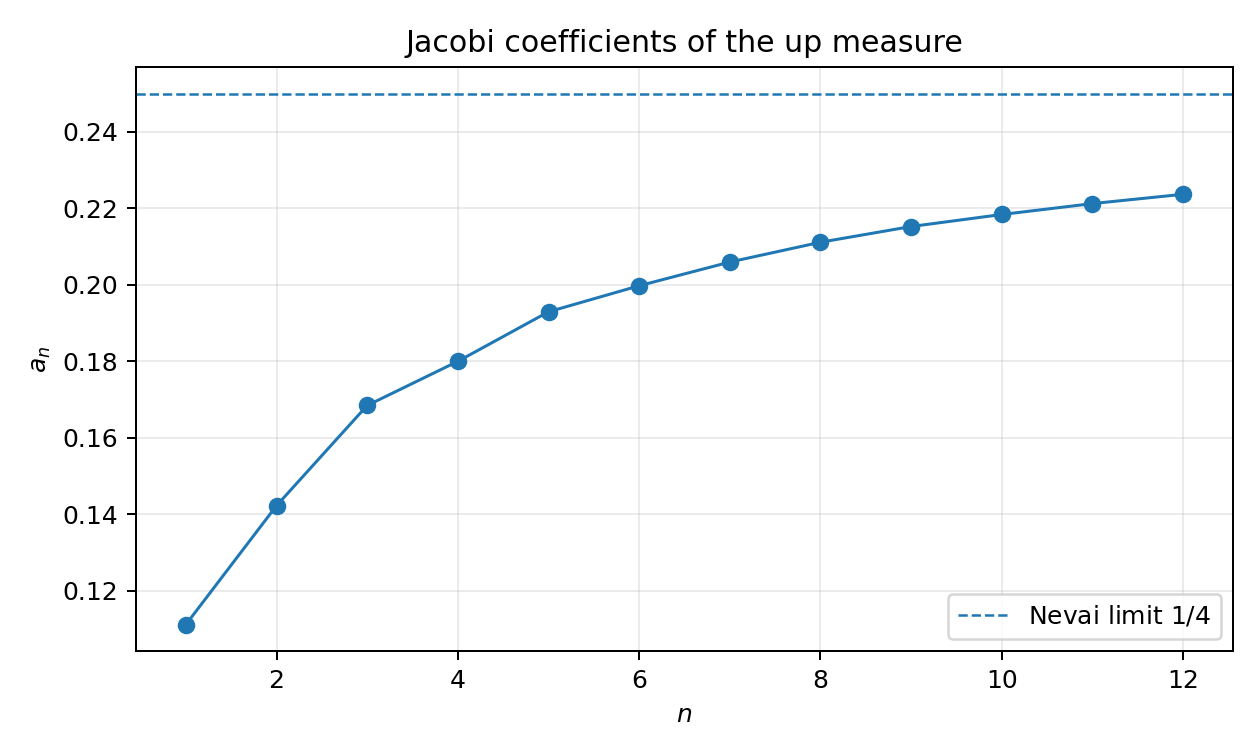
\includegraphics[width=0.78\textwidth]{jacobi_coefficients.png}
\caption{The first twelve exact Jacobi coefficients (shown in decimal form)
and the rigorous limiting value \(1/4\).  Monotonicity is suggested but not
proved.}
\label{fig:jacobi}
\end{figure}

\begin{conjecture}[Monotone Nevai approach]
\label{conj:jacobi-monotone}
The monic Jacobi coefficients of the up-law satisfy
\begin{equation}
 0<a_1<a_2<a_3<\cdots<\frac14.
 \label{eq:jacobi-monotone}
\end{equation}
\statusconjecture
\end{conjecture}

The first twelve coefficients support the conjecture, but endpoint flatness can
produce subtle high-order recurrence effects.  A proof may require total
positivity of suitable Hankel-ratio arrays, a comparison theorem for even
weights, or a direct use of \eqref{eq:Cauchy-functional} in Jacobi coordinates.

% --------------------------------------------------------------------------
\section{Nonlinear powers and order statistics}
\label{sec:power-integrals}

\subsection{Exact order-statistic identities}

Let \(X_1,X_2,\ldots\) be independent copies of \(X\), and let
\(\QF=F^{-1}\).

\begin{theorem}[Power integrals as minima]
\label{thm:power-minimum}
For every integer \(p\ge1\),
\begin{equation}
 \boxed{
 \int_0^1\Up(x)^p\dd x
 =\int_0^1F(x)^p\dd x
 =\E\min(X_1,\ldots,X_p).}
 \label{eq:power-minimum}
\end{equation}
Equivalently,
\begin{equation}
 \boxed{
 \int_0^1\Up(x)^p\dd x
 =p\int_0^1\QF(v)(1-v)^{p-1}\dd v.}
 \label{eq:power-beta-quantile}
\end{equation}
\statusproved
\end{theorem}

\begin{proof}
The survival function of the minimum is \(\Up(x)^p\), so its expectation is the
first integral.  Reflection gives \(\int F^p=\int\Up^p\).  If
\(B_p=\min(U_1,\ldots,U_p)\) for uniform variables, then
\(B_p\) has density \(p(1-v)^{p-1}\), and
\(\min(X_1,\ldots,X_p)\stackrel d=\QF(B_p)\).
\end{proof}

\begin{theorem}[Mixed powers as a random gap]
\label{thm:mixed-powers-gap}
Let \(m,n\ge1\), let
\(A=\max(X_1,\ldots,X_m)\), and let
\(B=\min(X_{m+1},\ldots,X_{m+n})\).  Then
\begin{equation}
 \boxed{
 \int_0^1F(x)^m\Up(x)^n\dd x=\E(B-A)_+.}
 \label{eq:mixed-gap}
\end{equation}
\statusproved
\end{theorem}

\begin{proof}
For fixed \(x\), \(F(x)^m\Up(x)^n=\Prob(A\le x<B)\).  Integrate the indicator
over \(x\in[0,1]\) and use Fubini.
\end{proof}

Fractional exponents are linked to the inverse without introducing a
noninteger number of samples: \eqref{eq:power-fractional-bridge} gives
\begin{equation}
 \int_0^1\Up(x)^\alpha\dd x
 =\Gamma(\alpha+1)(I_{0+}^{\alpha}\QF)(1),
 \qquad \alpha>0.
 \label{eq:power-alpha-Q}
\end{equation}

\subsection{Large-power asymptotics from inverse slow variation}

The inverse-frontier corpus proves the endpoint elasticity
\cite{proveitInverse}
\begin{equation}
 \frac{u\QF'(u)}{\QF(u)}\longrightarrow0
 \qquad(u\downarrow0),
 \label{eq:Q-elasticity-zero}
\end{equation}
with a sharper lower-Lambert and periodic expansion.  It follows that \(\QF\)
is slowly varying at zero:
\begin{equation}
 \frac{\QF(cu)}{\QF(u)}\longrightarrow1
 \qquad(u\downarrow0),\quad c>0.
 \label{eq:Q-slow-variation}
\end{equation}

\begin{theorem}[Power-integral scale]
\label{thm:power-asymptotic}
As \(p\to\infty\) through positive integers,
\begin{equation}
 \boxed{
 \int_0^1\Up(x)^p\dd x\sim\QF(1/p).}
 \label{eq:power-asymptotic}
\end{equation}
\statusproved
\end{theorem}

\begin{proof}
From \eqref{eq:power-beta-quantile}, substitute \(v=t/p\):
\[
 \frac{\int_0^1\Up(x)^p\dd x}{\QF(1/p)}
 =\int_0^p
 \frac{\QF(t/p)}{\QF(1/p)}
 \left(1-\frac tp\right)^{p-1}\dd t.
\]
For fixed \(t>0\), slow variation gives convergence of the ratio to one, and
the beta kernel converges to \(\e^{-t}\).  Potter bounds for slowly varying
functions provide an integrable majorant after splitting at \(t=1\); the
far tail is exponentially negligible.  Dominated convergence gives
\(\int_0^\infty\e^{-t}\dd t=1\).
\end{proof}

\begin{figure}[htbp]
\centering
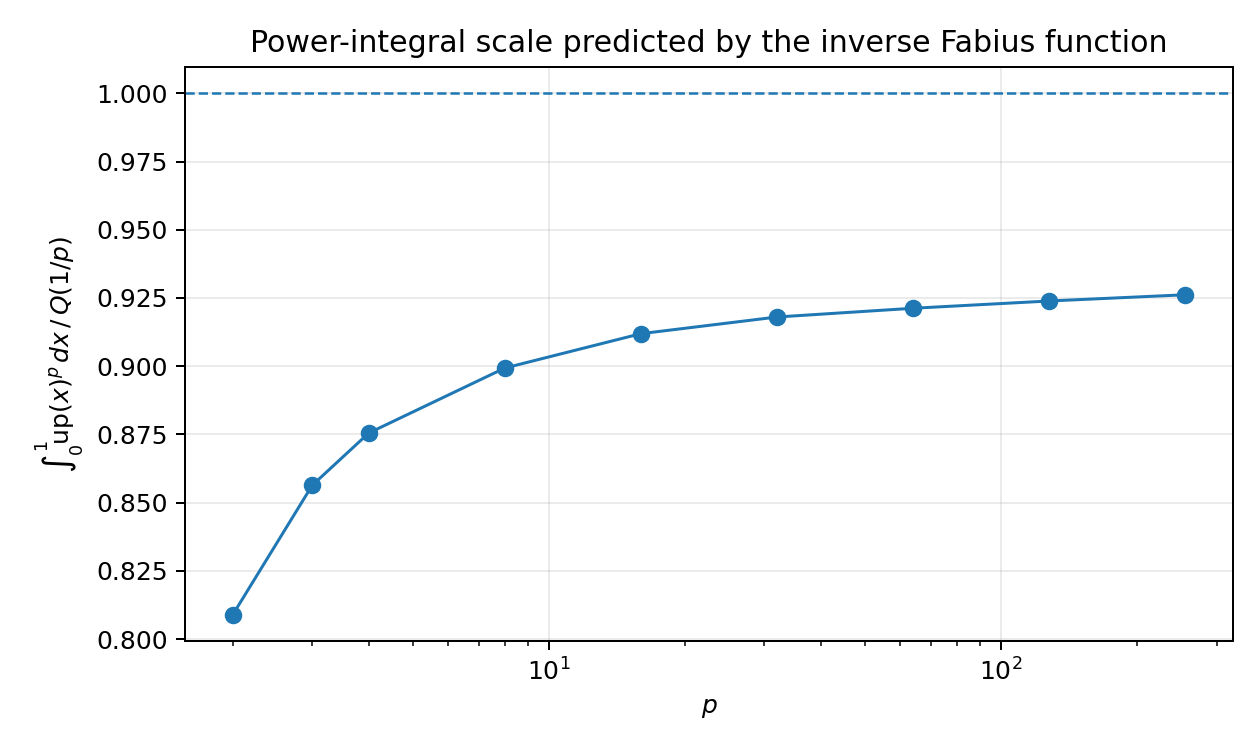
\includegraphics[width=0.78\textwidth]{power_quantile_ratio.png}
\caption{Numerical approach of
\(\int_0^1\Up(x)^p\dd x/\QF(1/p)\) toward the rigorous limit one.  The slow
approach reflects the lower-Lambert endpoint scale.}
\label{fig:power-ratio}
\end{figure}

Define the small elasticity
\begin{equation}
 h_p=\frac{p^{-1}\QF'(p^{-1})}{\QF(p^{-1})}.
 \label{eq:hp}
\end{equation}
The endpoint theory gives \(h_p\to0\), at a logarithmically slow rate.

\begin{proposition}[Conditional second-order law]
\label{prop:power-second-order}
Let \(B_p\) have the \(\mathrm{Beta}(1,p)\) law.  Assume the local
self-neglecting property
\begin{equation}
 \frac{tu\QF'(tu)/\QF(tu)}{u\QF'(u)/\QF(u)}\longrightarrow1
 \label{eq:self-neglecting-elasticity}
\end{equation}
uniformly for \(t\) in compact subsets of \((0,\infty)\), and assume that
the family
\begin{equation}
 Z_p=\frac{\QF(B_p)/\QF(1/p)-1}{h_p}
 \label{eq:Zp}
\end{equation}
is uniformly integrable.  Then
\begin{equation}
 \boxed{
 \int_0^1\Up(x)^p\dd x
 =\QF(1/p)\bigl(1-\gamma h_p+\smallo(h_p)\bigr),}
 \label{eq:power-second-order}
\end{equation}
where \(\gamma\) is Euler's constant.  More precisely,
\begin{equation}
 Z_p\Longrightarrow \log E,
 \qquad E\sim\mathrm{Exp}(1).
 \label{eq:power-logexp-limit}
\end{equation}
A second-order Potter bound dominating \(Z_p\) is one sufficient replacement
for the stated uniform-integrability assumption.  \statusconditional
\end{proposition}

\begin{proof}[Proof under the stated hypotheses]
Since \(pB_p\Rightarrow E\), integrate the logarithmic derivative of \(\QF\)
between \(1/p\) and \(t/p\).  The self-neglecting condition gives
\[
 \log\frac{\QF(t/p)}{\QF(1/p)}=h_p\log t+\smallo(h_p)
\]
locally uniformly.  Exponentiation yields the distributional limit.  The stated
uniform integrability permits passage to expectations, and
\(\E\log E=-\gamma\) gives \eqref{eq:power-second-order}.
\end{proof}

\begin{conjecture}[Second-order endpoint regularity]
The self-neglecting condition \eqref{eq:self-neglecting-elasticity} and the
required uniform integrability follow from the repository's all-orders inverse
lower-Lambert expansion, uniformly on every compact multiplicative \(t\)-range.
Consequently \eqref{eq:power-second-order} holds without an additional
hypothesis.
\statusconjecture
\end{conjecture}

% --------------------------------------------------------------------------
\section{Correlation and transform families}
\label{sec:correlation}

Although autocorrelation identities are standard Fourier consequences, they
provide useful definite integrals involving two copies of the up-function.
Define
\begin{equation}
 C(a)=\int_{\R}\Up(x)\Up(x+a)\dd x=(\Up*\Up)(a).
 \label{eq:autocorrelation}
\end{equation}
With the Fourier convention
\(\widehat f(\xi)=\int f(x)\e^{-2\pi\ii x\xi}\dd x\),
\begin{equation}
 \widehat C(\xi)=|\widehat\Up(\xi)|^2
 =\prod_{j=0}^{\infty}
 \sinc^2\!\left(\frac{\pi\xi}{2^j}\right).
 \label{eq:autocorrelation-fourier}
\end{equation}
Thus
\begin{equation}
 C(a)=\int_{\R}
 \prod_{j=0}^{\infty}
 \sinc^2\!\left(\frac{\pi\xi}{2^j}\right)
 \e^{2\pi\ii a\xi}\dd\xi.
 \label{eq:autocorrelation-inverse}
\end{equation}
More generally,
\begin{equation}
 \int_{\R}\Up^{(m)}(x)\Up^{(n)}(x+a)\dd x
 =\int_{\R}(-2\pi\ii\xi)^m(2\pi\ii\xi)^n
 |\widehat\Up(\xi)|^2\e^{2\pi\ii a\xi}\dd\xi.
 \label{eq:derivative-correlation}
\end{equation}
At \(a=0\),
\begin{equation}
 \|\Up^{(m)}\|_2^2
 =(2\pi)^{2m}\int_{\R}\xi^{2m}
 \prod_{j=0}^{\infty}
 \sinc^2\!\left(\frac{\pi\xi}{2^j}\right)\dd\xi.
 \label{eq:Sobolev-energy}
\end{equation}
These formulae turn Sobolev energies and shifted derivative overlaps into
integral transforms of the squared infinite sinc product.  The corpus's Fourier
decay theory supplies convergence at every derivative order.

% --------------------------------------------------------------------------
\section{Numerical verification and reproducibility}
\label{sec:numerics}

\subsection{Exact and floating-point layers}

The companion program \path{numerical_experiments.py} separates proof from
experiment.
\begin{enumerate}
\item Bernoulli cumulants, moments, Gram polynomials, and Jacobi coefficients
      are computed with Python's exact \texttt{Fraction} arithmetic.
\item A uniform grid on \([-1,1]\) is iterated under the positive fixed-point
      operator
      \[
        (Tg)(x)=\int_{2x-1}^{2x+1}g(t)\dd t.
      \]
      The resulting density is used only to cross-check analytic identities.
\item Adaptive or grid quadrature checks the Cauchy equation, fractional
      refinement, inverse fractional layer cake, order-statistic formulae, and
      generalized-moment Newton series.
\end{enumerate}

With 65,537 grid points and 25 refinement iterations, the main diagnostics were
\begin{center}
\small
\begin{tabularx}{0.95\textwidth}{@{}Xr@{}}
\toprule
Check & observed residual / error \\
\midrule
Mass of reconstructed \(\Up\) & \(2.2\times10^{-16}\) from one \\
Variance versus exact \(1/9\) & \(5.2\times10^{-11}\) \\
Maximum symmetry defect & \(1.5\times10^{-14}\) \\
Cauchy equation at three complex points & relative \(2.9\times10^{-11}\) to \(5.6\times10^{-11}\) \\
Fractional up-refinement & \(1.3\times10^{-12}\) to \(7.7\times10^{-7}\) \\
Inverse fractional identity & \(9.4\times10^{-11}\) to \(1.3\times10^{-8}\) \\
Newton series for \(m(-1/2),m(1/2),m(3/2)\) & \(3.3\times10^{-8}\) to \(8.0\times10^{-12}\) \\
Logarithmic identity \(\int F(x)/x\dd x=-m'(0)\) & \(4.4\times10^{-9}\) \\
\bottomrule
\end{tabularx}
\end{center}

\begin{figure}[htbp]
\centering
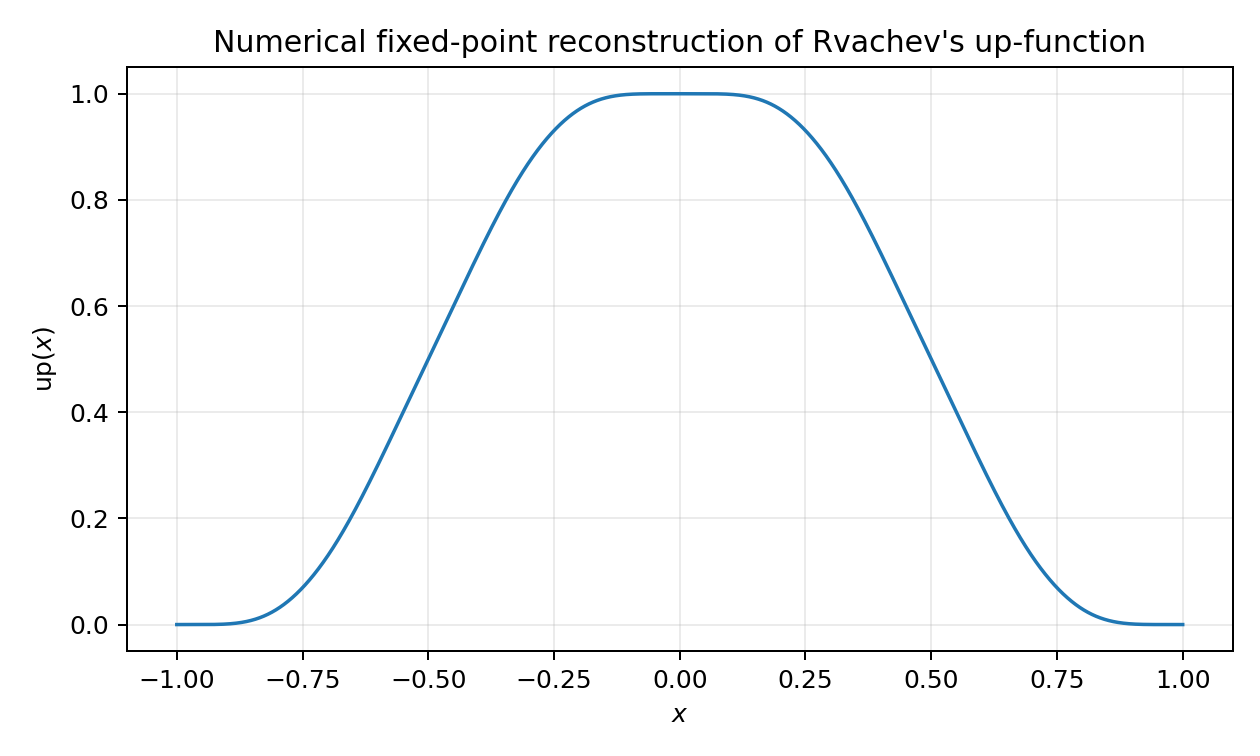
\includegraphics[width=0.78\textwidth]{up_reconstruction.png}
\caption{Positive fixed-point reconstruction used for numerical cross-checks.
The exact theory, not this discretization, is the source of all theorems.}
\label{fig:up-reconstruction}
\end{figure}

The full exact fractions through \(a_{12}\), every test point, precision
setting, and residual are recorded in \path{experiments_summary.txt}.  The
script is deterministic and uses no Monte Carlo simulation.

\subsection{Reproduction command}

From the extracted archive directory:
\begin{lstlisting}[style=reportcode]
python numerical_experiments.py --output-dir reproduced
latexmk -pdf -interaction=nonstopmode -halt-on-error \
  Fabius_Integral_Transform_Fractional_Frontiers.tex
\end{lstlisting}
The generated table \path{jacobi_coefficients.tex} and all three figures are
included in the PDF build.

% --------------------------------------------------------------------------
\section{Conjectures and future research directions}
\label{sec:future}

\subsection{Cauchy renormalization as a spectral equation}

Equation \eqref{eq:Cauchy-functional} deserves treatment as a boundary-value
renormalization problem in its own right.

\begin{problem}[Uniqueness from analytic data]
Characterize the weakest growth and Herglotz conditions under which
\[
 S'(z)=2[S(2z+1)-S(2z-1)],\qquad S(z)\sim z^{-1},
\]
uniquely determines the up-law.  A positive answer would provide a transform-
space definition of \(\Up\) independent of the infinite convolution.
\end{problem}

\begin{problem}[Dyadic Pad\'e acceleration]
Combine the J-fraction convergents with the affine values
\(S(2z\pm1)\) in \eqref{eq:Cauchy-functional} to build certified rational
approximants on \(\C\setminus[-1,1]\).  Determine whether the dyadic equation
improves the usual Markov convergence bounds for Stieltjes continued fractions.
\end{problem}

\subsection{Jacobi arithmetic and endpoint flatness}

The exact rational coefficients \(a_n\) form a new arithmetic sequence attached
to the up-law.  Beyond \cref{conj:jacobi-monotone}, natural questions are:
\begin{enumerate}
\item determine sharp denominator-clearing products in terms of Mersenne
      factors \(2^k-1\) or \(4^k-1\);
\item find the first correction to \(a_n=1/4+o(1)\), and decide whether endpoint
      flatness produces a logarithmic, stretched-exponential, or oscillatory
      rate;
\item translate the Cauchy functional equation into a closed hierarchy for
      Jacobi parameters or Hankel ratios;
\item construct a Lean proof of the first exact coefficients from the already
      formalized rational moment recurrence.
\end{enumerate}

\subsection{Fractional endpoint asymptotics}

The repository's endpoint expansion controls \(F(x)\) and \(Q(u)\) through a
lower-Lambert variable and periodic Gamma--zeta terms.  The expectation kernels
in \eqref{eq:F-fractional-integral}, \eqref{eq:weighted-F-fractional}, and
\eqref{eq:Q-fractional-integral} suggest a larger transseries.

\begin{conjecture}[Fractional lower-Lambert transseries]
For fixed noninteger \(\alpha>0\), the endpoint asymptotic expansions of
\(I_{0+}^{\alpha}F\), \(D_{0+}^{\alpha}F\), and
\(I_{0+}^{\alpha}Q\) are organized by the same exact lower-Lambert phase as
\(F\) and \(Q\), with coefficients obtained by beta/gamma shifts of the
existing periodic saddle jets.
\statusconjecture
\end{conjecture}

A practical route is to insert the known endpoint density expansion into the
truncated-power expectations, split at the saddle scale, and carry the beta
kernel through the existing uniform remainder estimates.

\subsection{Nonlinear power integrals}

The first-order equivalence \eqref{eq:power-asymptotic} is rigorous.  The next
frontier is to prove the self-neglecting property required in
\cref{prop:power-second-order} and then propagate the complete inverse
transseries through the beta kernel.  This should produce
\begin{equation}
 \int_0^1\Up(x)^p\dd x
 =\QF(1/p)\left(1-\gamma h_p+c_2h_p^2+	ext{periodic corrections}+\cdots\right),
 \label{eq:power-full-frontier}
\end{equation}
where \(c_2\) should involve moments of \(\log E\), hence \(\pi^2/6\) and
\(\gamma^2\), while the periodic terms inherit the Gamma--zeta phase of the
inverse Fabius expansion.

\subsection{Fractional formalization roadmap}

\begin{obligation}[Kernel layer]
Formalize Tonelli identities for survival functions and quantiles, including
\cref{thm:survival-kernel,thm:inverse-layercake}.  These are measure-theoretic
but structurally short.
\end{obligation}

\begin{obligation}[Special-function layer]
Introduce incomplete beta integrals and prove
\cref{thm:weighted-fractional-master} first for positive real parameters.
Complex continuation can remain outside the initial formalization.
\end{obligation}

\begin{obligation}[Transform layer]
Build the Cauchy transform off a compact interval, justify differentiation and
integration by parts, and formalize \eqref{eq:Cauchy-functional}.  The proof
uses only the already established up refinement equation and compact support.
\end{obligation}

\begin{obligation}[Orthogonal-polynomial layer]
Reuse the corpus's Hankel-positivity and Gaussian-quadrature infrastructure to
construct \(a_n=h_n/h_{n-1}\), the finite J-fraction convergents, and exact
certificates for the first coefficients.  Rakhmanov's asymptotic theorem may be
imported as a separately documented analytic dependency.
\end{obligation}

% --------------------------------------------------------------------------
\section{Conclusion}
\label{sec:conclusion}

The Fabius--Rvachev system admits a broader integral calculus than its original
differential and Fourier definitions suggest.  Three probability identities
supply the organizing principle:
\begin{equation}
 \Up(x)=\Prob(X>x),
 \qquad
 F(x)=\Prob(X\le x),
 \qquad
 \QF(u)=\inf\{x:F(x)\ge u\}.
 \label{eq:three-probability-objects}
\end{equation}
From them follow:
\begin{enumerate}
\item arbitrary-kernel and monomial antiderivatives as truncated moments;
\item an entire generalized-moment function reconstructed from rational moments
      by a Newton series;
\item a Mellin triad distinguishing the single pole of \(\Up\) from the entire
      transforms of \(F\) and \(F'\);
\item exact layer-cake transforms and fractional derivatives of the inverse;
\item incomplete-beta formulae interpolating ordinary, repeated, negative-power,
      and fractional antiderivatives;
\item a Cauchy functional-differential equation and the explicit Jacobi fraction
      requested by an existing frontier report;
\item order-statistic interpretations and a sharp inverse-Fabius scale for
      nonlinear power integrals.
\end{enumerate}

The most promising next step is to combine the new kernel formulae with the
repository's all-orders lower-Lambert endpoint theory.  That synthesis should
turn several conditional statements here---especially the second-order power
integral and fractional endpoint transseries---into explicit theorems with
periodic Gamma--zeta coefficients.

\appendix

% --------------------------------------------------------------------------
\section{Exact formula sheet}
\label{app:formula-sheet}

\begin{longtable}{@{}p{0.29\textwidth}p{0.66\textwidth}@{}}
\toprule
Object & Exact formula \\
\midrule
\endfirsthead
\toprule
Object & Exact formula \\
\midrule
\endhead
Fabius moment
& \(m(s)=\E X^s=\sum_{n\ge0}(-1)^n\binom{s}{n}m_n\) \\
Mellin of positive up-half
& \(\int_0^1x^{s-1}\Up(x)\dd x=m(s)/s\) \\
Mellin of \(F\)
& \(\int_0^1x^{s-1}F(x)\dd x=(1-m(s))/s\) \\
Monomial up integral
& \(\int_0^1x^p\Up(x)\dd x=m(p+1)/(p+1)\), \(\Re p>-1\) \\
Monomial Fabius integral
& \(\int_0^1x^pF(x)\dd x=(1-m(p+1))/(p+1)\), entire in \(p\) \\
Laplace/exponential up-half
& \(\int_0^1\Up(x)\e^{zx}\dd x=(A(z)-1)/z\) \\
Laplace/exponential Fabius
& \(\int_0^1F(x)\e^{zx}\dd x=(\e^z-A(z))/z\) \\
Quantile moments
& \(\int_0^1\QF(u)^p\dd u=m(p)\) \\
Inverse primitive
& \(\int_0^u\QF(v)\dd v=u\QF(u)-\int_0^{\QF(u)}F(x)\dd x\) \\
Fractional \(F\) primitive
& \(I_{0+}^{\alpha}F(x)=\E(x-X)_+^\alpha/\Gamma(\alpha+1)\) \\
Fractional inverse primitive
& \(I_{0+}^{\alpha}\QF(u)=\Gamma(\alpha+1)^{-1}\int_0^{\QF(u)}(u-F(x))^\alpha\dd x\) \\
Power/fractional bridge
& \(\int_0^1\Up(x)^\alpha\dd x=\Gamma(\alpha+1)I_{0+}^{\alpha}\QF(1)\) \\
Cauchy equation
& \(S'(z)=2[S(2z+1)-S(2z-1)]\) \\
Jacobi fraction
& \(S(z)=1/(z-a_1/(z-a_2/(z-\cdots)))\), \(a_n\in\mathbb Q_{>0}\), \(a_n\to1/4\) \\
Power asymptotic
& \(\int_0^1\Up(x)^p\dd x\sim\QF(1/p)\) \\
\bottomrule
\end{longtable}

% --------------------------------------------------------------------------
\section{Corpus families inspected}
\label{app:corpus}

The recursive audit was organized by mathematical lineage.  The principal
families were:
\begin{enumerate}
\item the living primary exposition \emph{Fabius Function and Rvachev Up};
\item the mathematical glossary, non-elementarity article, and Lean walkthrough;
\item the consolidated non-formalized frontier volume and provenance/gap register;
\item repeated-integration and up-from-integration manuscripts;
\item dyadic formula, \(q\)-connection, asymptotic bridge, and small-argument
      manuscripts;
\item inverse-function, inverse-saddle, and lower-Lambert reports;
\item the Thue--Morse formula atlas and its archived drafts;
\item active arithmetic-ray, self-sampling, half-integer spectral, exponent-
      sequence/Newton, spectral-Pascal, finite-block, sinc-Richardson, and
      Fourier-decay reports;
\item imported TeX sources for the classical Fabius, Rvachev, arithmetic, and
      compact-support literature;
\item frozen archive variants retained by the repository's provenance map.
\end{enumerate}
The exact 67-path list at the pinned commit is recorded in the inventory appendix
of the exponent-sequence/Newton report \cite{proveitNewton}.  Current descendants
and newly active draft folders were rechecked separately so that the audit did
not stop at the pinned snapshot.

% --------------------------------------------------------------------------
\section{Reproducibility manifest}
\label{app:manifest}

The companion ZIP archive contains:
\begin{center}
\begin{tabularx}{0.96\textwidth}{@{}p{0.42\textwidth}X@{}}
\toprule
Path & Purpose \\
\midrule
\path{Fabius_Integral_Transform_Fractional_Frontiers.tex}
& Complete LaTeX manuscript \\
\path{Fabius_Integral_Transform_Fractional_Frontiers.pdf}
& Compiled and visually inspected report \\
\path{numerical_experiments.py}
& Commented exact/numerical verification program \\
\path{experiments_summary.txt}
& Full deterministic diagnostics and exact coefficients \\
\path{jacobi_coefficients.tex}
& Generated exact table used in the manuscript \\
\path{up_reconstruction.png}
& Fixed-point density diagnostic \\
\path{jacobi_coefficients.png}
& Exact-coefficient trend figure \\
\path{power_quantile_ratio.png}
& Power-integral asymptotic diagnostic \\
\path{requirements.txt}
& Python package versions used \\
\path{README.md}
& Build and reproduction instructions \\
\path{SHA256SUMS}
& Checksums for packaged artifacts \\
\bottomrule
\end{tabularx}
\end{center}

% --------------------------------------------------------------------------
\begin{thebibliography}{99}

\bibitem{proveitPrimary}
V.~Reshetnikov,
\newblock \emph{Fabius Function and Rvachev Up}, living primary exposition,
\newblock in the \texttt{ProveIt} repository, \path{Analysis/FabiusFunction/docs}, accessed 27 August 2026.

\bibitem{proveitFrontiers}
V.~Reshetnikov,
\newblock \emph{Fabius Function Research Frontiers}, consolidated non-formalized frontier volume,
\newblock \texttt{ProveIt} repository, accessed 27 August 2026.

\bibitem{proveitFrontierReadme}
V.~Reshetnikov,
\newblock \emph{Non-formalized research frontiers: quarantine and provenance README},
\newblock \texttt{ProveIt} repository, accessed 27 August 2026.

\bibitem{proveitArchive}
V.~Reshetnikov,
\newblock \emph{Fabius documentation archive and provenance catalogue},
\newblock \texttt{ProveIt} repository, accessed 27 August 2026.

\bibitem{proveitQuadrature}
\emph{Tail Quadrature, Exact Dyadic Error Laws, and $q$-Binomial Acceleration for the Fabius--Rvachev System},
\newblock active frontier report in the \texttt{ProveIt} repository, 27 August 2026.

\bibitem{proveitInverse}
\emph{Inverse Frontiers for the Fabius--Rvachev System},
\newblock active frontier report in the \texttt{ProveIt} repository, 27 August 2026.

\bibitem{proveitNewton}
\emph{Exponent-Sequence and Newton-Basis Frontiers for the Fabius--Rvachev System},
\newblock active frontier report and 67-source audit inventory,
\newblock commit \texttt{32d6d36c51d803289e6d6a0dc0c37753766eba47}, 27 August 2026.

\bibitem{fabius1966}
J.~Fabius,
\newblock A probabilistic example of a nowhere analytic $C^\infty$-function,
\newblock \emph{Zeitschrift f\"ur Wahrscheinlichkeitstheorie und Verwandte Gebiete}
\textbf{5} (1966), 173--174.

\bibitem{rvachev1990}
V.~A.~Rvachev,
\newblock Compactly supported solutions of functional-differential equations and their applications,
\newblock \emph{Russian Mathematical Surveys} \textbf{45} (1990), no.~1, 87--120.

\bibitem{arias1982}
J.~Arias de Reyna,
\newblock Definici\'on y estudio de una funci\'on indefinidamente diferenciable de soporte compacto,
\newblock \emph{Revista de la Real Academia de Ciencias Exactas, F\'isicas y Naturales de Madrid}
\textbf{76} (1982), no.~1, 21--38;
\newblock English translation, arXiv:1702.05442.

\bibitem{ariasArithmetic}
J.~Arias de Reyna,
\newblock Arithmetic of the Fabius function,
\newblock \emph{INTEGERS} \textbf{18} (2018), Article A51; arXiv:1702.06487.

\bibitem{samko}
S.~G.~Samko, A.~A.~Kilbas, and O.~I.~Marichev,
\newblock \emph{Fractional Integrals and Derivatives: Theory and Applications},
\newblock Gordon and Breach, 1993.

\bibitem{podlubny}
I.~Podlubny,
\newblock \emph{Fractional Differential Equations},
\newblock Academic Press, 1999.

\bibitem{simonSzego}
B.~Simon,
\newblock \emph{Szeg\H{o}'s Theorem and Its Descendants: Spectral Theory for $L^2$ Perturbations of Orthogonal Polynomials},
\newblock Princeton University Press, 2011.

\bibitem{shoHatTamarkin}
J.~A.~Shohat and J.~D.~Tamarkin,
\newblock \emph{The Problem of Moments},
\newblock American Mathematical Society, 1943.

\bibitem{bingham}
N.~H.~Bingham, C.~M.~Goldie, and J.~L.~Teugels,
\newblock \emph{Regular Variation},
\newblock Cambridge University Press, 1987.

\bibitem{deHaanFerreira}
L.~de Haan and A.~Ferreira,
\newblock \emph{Extreme Value Theory: An Introduction},
\newblock Springer, 2006.

\end{thebibliography}

\end{document}
